% !TeX root = ../main.tex
% 修改稿迁移版：自动编号，原文数据与待核事项保留。
\chapter{运营分析}
PI OS 的运营目标，是将已经完成的代码开发成果转化为可部署、可验收、可持续维护的企业级产品。项目将围绕“质量可靠、交付可控、成本清晰、责任明确”建立运营机制，先完成企业命题验证，再推进客户试点与商业化交付。

德勤于 2026 年 8 月发布的调查显示，67\% 的受访管理者认为智能体集成成本过高、过程复杂，70\% 表示对智能体的信任与治理能力存在顾虑。该调查于 2026 年 4---6 月开展，覆盖美国五个行业的 501 名管理者，参与企业均已至少开展智能体试点。上述结果反映出，企业落地智能体不仅需要技术产品，还需要配套的部署、质量和服务管理。

以下质量制度与组织安排为 PI OS 拟实施的运营方案，创业后的部门和岗位根据实际业务逐步建立。

\section{质量评审}\label{sec:5.1}
PI OS 的质量评审对象包括运行引擎、系统适配代码、部署工具、测试结果和交付文档。评审重点是：能否满足企业指定条件、正确完成任务，以及客户接入后能否稳定使用。

项目拟建立“开发自检、交叉复核、场景验收”三级质量机制。开发人员负责模块自检，其他成员复核关键功能和实验结果，最终依据企业命题或客户约定完成场景验收。影响任务正确性、资源限制和数据隔离的重大问题未解决前，不进入正式交付。

\begin{figure}[H]\centering
\setcounter{figure}{0}
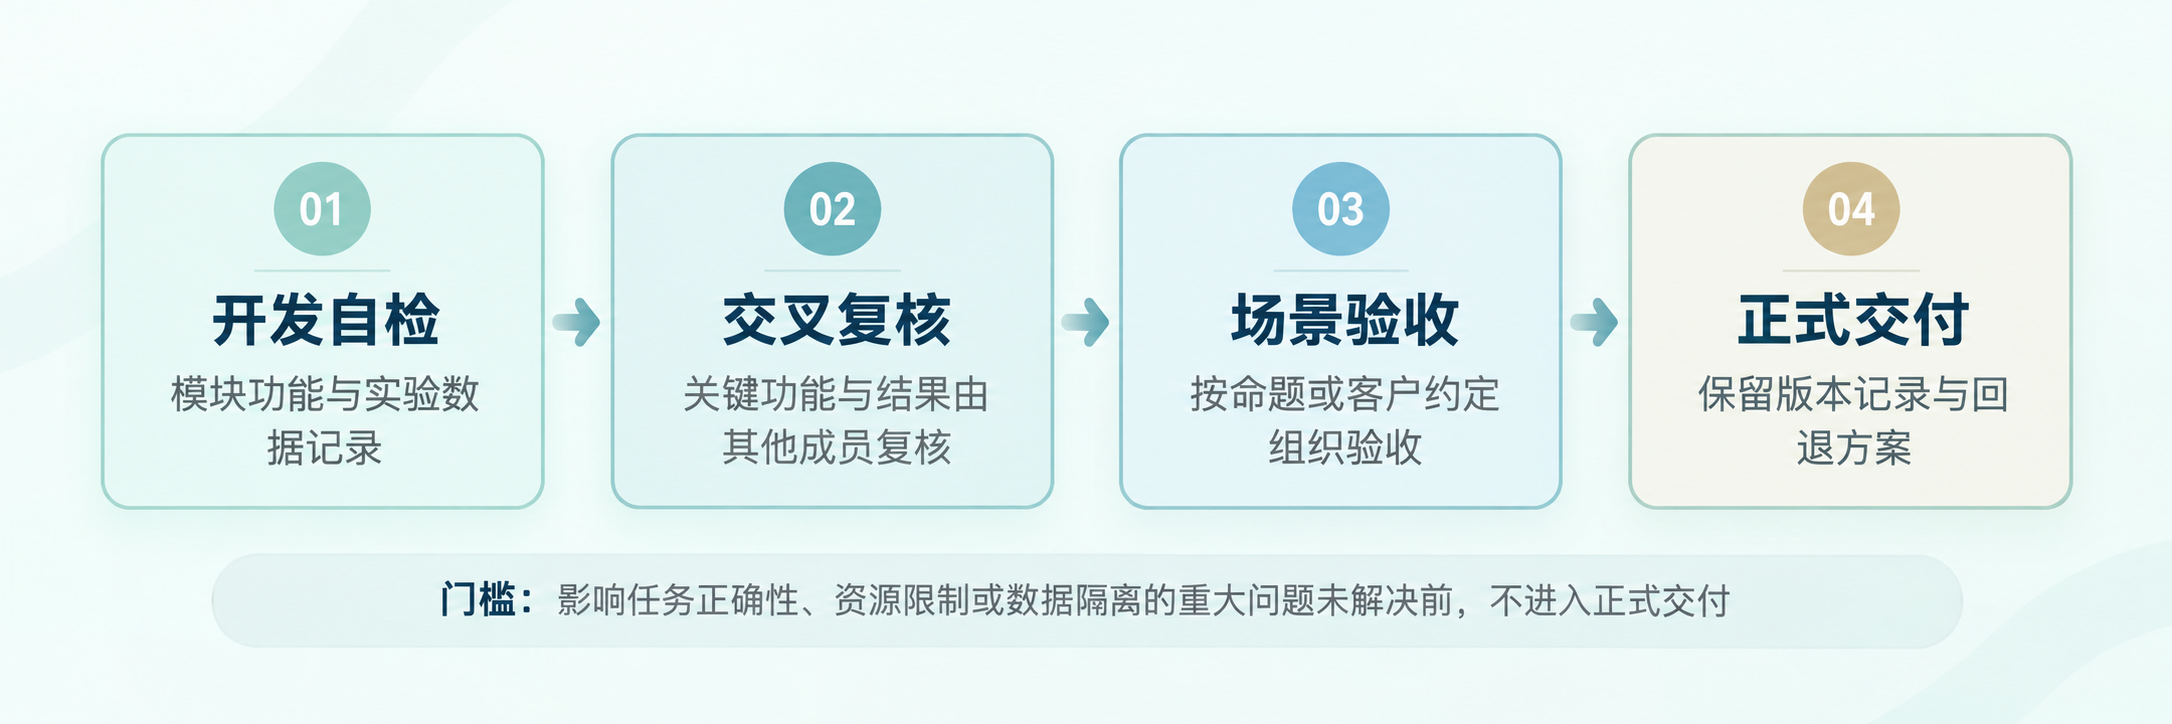
\includegraphics[width=\linewidth,height=.50\textheight,keepaspectratio]{figures/updated-5-1.png}
\caption{三级质量评审流程}\label{fig:5-1}
\end{figure}
按照华为命题的技术评价要求，PI OS 的质量工作安排见表 5-1。

\FloatBarrier
\begingroup\linespread{1}\selectfont
\setcounter{table}{0}
\begin{table}[H]\centering
\caption{企业命题技术评价与质量工作对应关系}\label{tab:5-1}
\color{TableText}\fontsize{9pt}{12.6pt}\selectfont
\begin{tabular}{@{}>{\raggedright\arraybackslash}p{\dimexpr 0.15950\linewidth-0.9570\tabcolsep\relax}>{\raggedright\arraybackslash}p{\dimexpr 0.11724\linewidth-0.7034\tabcolsep\relax}>{\raggedright\arraybackslash}p{\dimexpr 0.40427\linewidth-2.4256\tabcolsep\relax}>{\raggedright\arraybackslash}p{\dimexpr 0.31900\linewidth-1.9140\tabcolsep\relax}@{}}
\hline
\rowcolor{WordTableHeader} \TableHeaderText{技术评价项} & \TableHeaderText{权重} & \TableHeaderText{PI OS 质量工作重点} & \TableHeaderText{主要验收材料} \\ \hline
\rowcolor{WordTableStripe} 
功能完整性 & 35\% & 指定环境运行、任务执行、资源管理及异常处理 & 功能测试记录、任务结果、演示材料 \\ \hline
性能满足度 & 30\% & 在规定资源条件下验证有效并发、完成时间和稳定性 & 对照实验、资源记录、统计结果 \\ \hline
\rowcolor{WordTableStripe} 
创新性和代码质量 & 25\% & 验证三项方案的实际贡献，检查代码结构与维护能力 & 分项实验、代码审查和版本记录 \\ \hline
文档完整性 & 10\% & 确保产品能够构建、部署、复现和排障 & 部署手册、测试报告、维护文档 \\ \hline
\end{tabular}
\end{table}\endgroup
\subsection{功能可行性}\label{sec:5.1.1}
\NumberedPara{1}{\textbf{命题条件符合性}}
质量评审首先检查企业指定的技术环境、资源限制和任务要求，以 openEuler/\allowbreak{}Conch + StratoVirt 代码和镜像为准，核对管理面与全部容器总内存不超过 16GB、每个沙箱内部可见规格为 2U8G、关闭 Swap 等条件是否落实。

所有辅助管理和状态处理组件的资源开销均纳入约定计量范围。内部研究环境的测试结果与企业指定环境的验收结果分别记录。

\NumberedPara{2}{\textbf{任务结果正确性}}
代码修复任务需要保留原始问题、修改内容和测试结果；功能开发任务需事先明确功能要求与验收用例。任务是否成功，以实际执行结果为依据，而非仅依据智能体生成的“完成说明”。

Anthropic 于 2026 年 1 月发布的智能体评估实践强调，应检查环境中的最终结果，并通过重复试验观察表现的稳定性。PI OS 拟据此将任务结果、执行过程与异常记录一并纳入评审。

\NumberedPara{3}{\textbf{性能与资源计量}}
性能评审同时记录有效并发数量、任务成功率、完成时间、内存峰值和失败原因。其中，有效并发是指在同一时间窗口内实际运行并满足任务要求的独立沙箱数量，不能用累计任务数量代替。

对照实验固定硬件、模型、任务、软件版本和超时条件，并保留重复测试结果。Anthropic 于 2026 年 2 月披露，在其 Terminal-Bench 2.0 内部实验中，仅调整资源配置（其余条件不变），最高与最低配置下的任务成功率相差 6 个百分点。这说明资源条件本身可能显著影响结果，必须与性能数据同时报告。

\NumberedPara{4}{\textbf{三项方案贡献验证}}
运行时扁平化、动态资源卸载和智能内存共享分别开展验证，再测试组合效果。

运行时扁平化重点检查基础运行开销是否减少；动态资源卸载同时检查释放效果和恢复等待；智能内存共享同时检查重复占用变化和任务隔离情况。通过逐项开启、关闭相关功能，区分各项方案带来的收益与额外成本。

\NumberedPara{5}{\textbf{安全与隔离}}
评审覆盖任务之间的文件访问、权限边界、网络访问和凭据使用，检查一个任务是否可能读取或修改其他任务的数据。

共享机制拟优先面向经许可的公共只读内容，客户私有文件、凭据和可写状态保持隔离。沙箱负责执行环境的隔离，涉及发送信息、修改业务数据等操作的授权，由上层业务系统与客户管理流程共同控制。

\NumberedPara{6}{\textbf{异常处理与恢复}}
测试覆盖模型调用超时、任务取消、状态保存失败、恢复失败、进程退出和网络中断等情形。每类异常应具有明确的记录、提示及处理方式。

对于可能产生外部影响的操作，恢复前检查其是否已经执行，防止重复提交。故障处理优先控制影响范围、保留必要记录，再依据预案恢复任务或交由人工处理。

\NumberedPara{7}{\textbf{稳定性与版本发布}}
产品发布前开展持续运行、批量任务和反复启停测试，检查资源是否能够正常回收。涉及资源管理、恢复或共享机制的修改，必须重新执行相关回归测试。

拟采用小范围上线方式，先在受控环境或有限任务中观察新版本表现，确认无明显退化后再扩大使用范围。每次发布保留版本记录与回退方案。

\NumberedPara{8}{\textbf{客户使用价值}}
客户验收除技术指标外，还应检查部署工作量、维护投入和任务综合成本。

质量评审将分别呈现执行基础设施、模型调用、存储网络及运维成本，判断性能改善是否能够转化为客户可获得的经济收益。客户是否继续采购，以其真实使用结果和预算决策为依据。

\subsection{文档标准性}\label{sec:5.1.2}
PI OS 拟将文档作为产品交付的一部分，与代码版本同步管理。文档质量主要从完整性、正确性和一致性三个方面评审。

\NumberedPara{1}{\textbf{完整性}}
交付资料应覆盖环境要求、安装部署、使用接口、测试复现、故障处理和版本升级等内容。

部署文档说明所需设备、软件版本及配置步骤；测试文档列明任务、条件、指标定义与结果；维护文档提供常见问题、已知限制和回退方法，使接收方能够在约定支持范围内完成操作。

\NumberedPara{2}{\textbf{正确性}}
关键命令、配置步骤和测试流程由非原作者成员按照文档复核。图表标明数据来源、单位、样本数量和测试条件，计算结果能够追溯至原始记录。

实测结果、测算结果和后续目标分别标注，避免把预期效果写成已经完成的成果。

\NumberedPara{3}{\textbf{一致性}}
代码、镜像、配置、测试报告和使用手册使用统一版本标识。接口或配置发生变化时，同步更新相关资料，避免客户依据旧文档部署新版本。

面向企业验收、赛事展示和客户交流的材料统一采用经确认的数据口径，并按授权范围处理客户信息及合作资料。

\section{组织管理}\label{sec:5.2}
\subsection{创业初期}\label{sec:5.2.1}
创业初期以完成命题验证、形成标准交付包和开展客户试点为主要任务，采用项目负责人统筹、职能小组协作的管理方式。项目已完成代码开发，现阶段资源将重点投入适配验证、质量完善和交付准备。

\NumberedPara{1}{\textbf{按里程碑推进工作}}
将工作划分为需求确认、环境适配、质量验证、试点交付和问题复盘等阶段。每个阶段明确负责人、交付物、资源预算和验收条件，完成情况以代码、记录和实际结果确认。

拟每周检查进度与阻塞问题，每月复核预算、质量和客户反馈，及时调整优先级。

\begin{figure}[H]\centering
\setcounter{figure}{1}
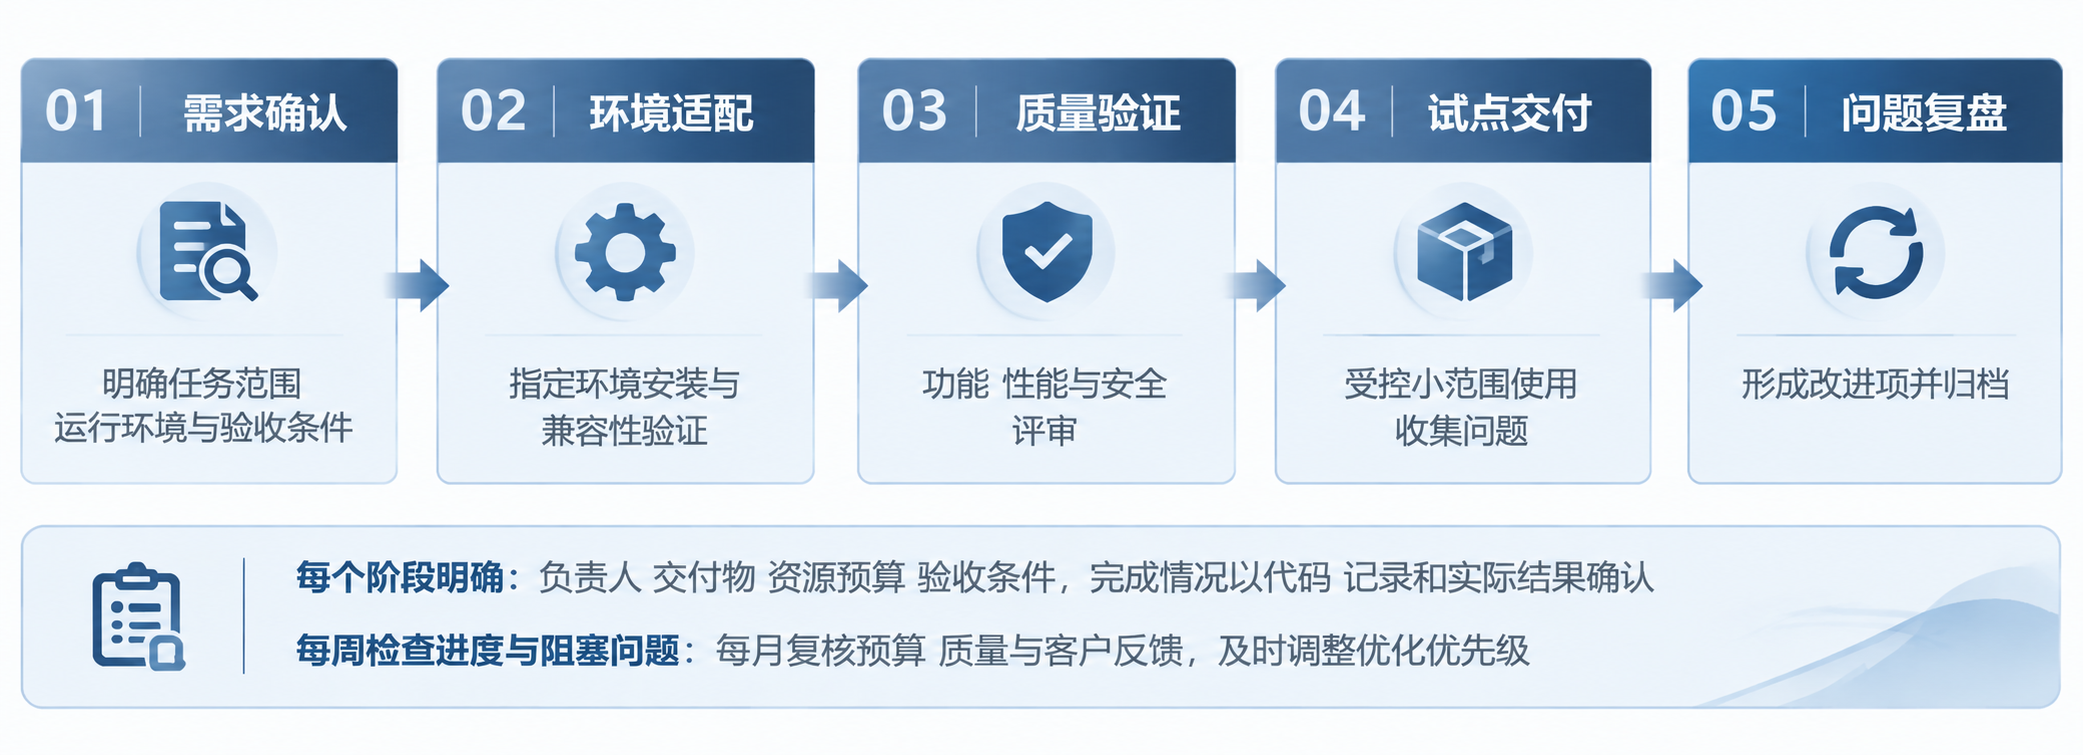
\includegraphics[width=\linewidth,height=.50\textheight,keepaspectratio]{figures/updated-5-2.png}
\caption{创业初期里程碑推进安排}\label{fig:5-2}
\end{figure}
\NumberedPara{2}{\textbf{明确客户交付范围}}
客户试点开始前，确认任务类型、运行环境、测试周期、验收指标和双方责任。新增需求先评估工作量及维护成本，再决定进入标准版本、单独报价或暂缓实施。

通过明确交付范围，控制免费验证和定制开发的投入，减少项目延期与重复返工。

\NumberedPara{3}{\textbf{分级处理运行问题}}
影响大范围任务或涉及数据隔离的问题，优先限制影响并升级处理；影响部分功能的问题，提供临时方案并安排修复；一般体验问题进入版本计划。

具体服务时段和响应承诺根据实际人员配置与合同确定，不在尚未建立保障能力时承诺全天候服务。

\NumberedPara{4}{\textbf{控制资金与资源投入}}
初期优先使用经授权的现有测试资源和客户部署环境，避免在需求尚未验证前大量采购设备。商业项目分别记录人工、云资源和外部服务支出，结合验收与付款节点安排投入。

科研经费、创业经营资金和客户款项按各自用途分别管理，不将科研合作合同金额直接视为创业主体可支配现金。

\subsection{创业成长期}\label{sec:5.2.2}
当试点能够转化为重复采购、交付流程逐步稳定后，项目进入以标准化和复制效率为重点的成长期。

\NumberedPara{1}{\textbf{推进产品与交付分工}}
研发侧维护通用产品、稳定版本和自动化测试；交付侧负责安装、接入和问题反馈。可复用的客户需求进入产品规划，单个客户的特殊需求单独管理。

通过减少重复开发，使新增客户数量增长不完全依赖研发人员同比增加。

\NumberedPara{2}{\textbf{建立运营指标记录}}
运营评价同时关注技术表现、客户转化和资金回收，拟采用以下指标。

\FloatBarrier
\begingroup\linespread{1}\selectfont
\setcounter{table}{1}
\begin{longtable}{@{}>{\raggedright\arraybackslash}p{\dimexpr 0.17999\linewidth-0.7200\tabcolsep\relax}>{\raggedright\arraybackslash}p{\dimexpr 0.60011\linewidth-2.4005\tabcolsep\relax}>{\raggedright\arraybackslash}p{\dimexpr 0.21990\linewidth-0.8796\tabcolsep\relax}@{}}
\caption{PI OS 拟跟踪的核心运营指标}\label{tab:5-2}\\
\hline
\rowcolor{WordTableHeader} \TableHeaderText{指标} & \TableHeaderText{统计口径} & \TableHeaderText{管理用途} \\ \hline
\endfirsthead
\multicolumn{3}{c}{\fontsize{9}{12}\selectfont 表 5-2（续）}\\
\hline
\rowcolor{WordTableHeader} \TableHeaderText{指标} & \TableHeaderText{统计口径} & \TableHeaderText{管理用途} \\ \hline
\endhead
\hline\endfoot\hline\endlastfoot
\rowcolor{WordTableStripe} 
有效任务成功率 & 满足预定验收条件的任务数占全部提交任务数的比例，另列失败原因 & 判断产品是否稳定可用 \\ \hline
试点付费转化率 & 已结束试点中转为付费合同的项目比例 & 检验客户需求与采购意愿 \\ \hline
\rowcolor{WordTableStripe} 
首次交付周期 & 从需求和环境确认至首次验收的时间 & 衡量接入效率 \\ \hline
单项目直接交付成本 & 实际交付人工、计算资源及外部服务等成本 & 识别低效定制与利润压力 \\ \hline
\rowcolor{WordTableStripe} 
客户续费率 & 统计期内到期客户中完成续费的比例 & 判断持续服务价值 \\ \hline
合同回款情况 & 按合同付款节点记录应收、实收与逾期情况 & 控制现金流风险 \\ \hline
\end{longtable}\endgroup
\NumberedPara{3}{\textbf{按业务瓶颈补充人员}}
人员扩充优先解决已经出现的交付瓶颈，例如测试积压、兼容问题或客户支持负担，而不是先建立完整部门再寻找业务。

新增岗位同时评估稳定工作量、收入支撑和现金储备，使组织规模与实际经营能力匹配。

\NumberedPara{4}{\textbf{逐步拓展合作交付}}
在产品接口、维护责任和成果授权明确后，探索与软件厂商、云服务商及系统集成商合作。合作前确认客户归属、支持边界、服务费用及问题升级机制，减少多方交付中的责任不清。

\subsection{创业成熟期}\label{sec:5.2.3}
当产品形成持续收入、稳定客户和可复制交付能力后，逐步建立专业化经营体系。

经营管理重点由单个项目推进转向产品生命周期、客户留存、成本效率和长期研发投入。公司治理及经营岗位根据实际主体和业务规模设置，必要时引入具有企业软件经营与交付经验的管理人员。

成熟期拟重点完善以下机制：

\NumberedPara{1}{\textbf{版本生命周期管理：明确版本支持期限、升级路径及停止维护安排。}}
\NumberedPara{2}{\textbf{服务质量管理：持续分析故障原因、恢复效果和客户反馈，减少同类问题反复发生。}}
\NumberedPara{3}{\textbf{经营预算管理：区分产品研发投入、客户交付成本和市场费用，定期检查投入产出。}}
\NumberedPara{4}{\textbf{客户与渠道管理：降低对单一客户、单一渠道或单一关键人员的依赖。}}
\NumberedPara{5}{\textbf{人才接续管理：通过文档、培训和岗位备份，保障人员变化后业务仍能持续运行。}}
\section{人事管理}\label{sec:5.3}
PI OS 的人员管理坚持职责明确、能力互补和贡献可追溯。参赛学生、科研合作人员与未来经营团队的身份分别记录，岗位规划不等同于现有劳动关系或任职事实。

企业命题组评审将“团队协作”列为 20 分评价项，并明确从团队结构、团队资源与团队贡献等方面考察。因此，团队建设既关注后续经营能力，也重视学生在需求调研、工程验证和项目协作中的真实成长。

\subsection{创业初期管理架构}\label{sec:5.3.1}
初期拟采用精简的职能协作架构，由项目负责人统筹，下设产品研发、质量验证、交付运营和商务综合四类职责。成员可以根据能力兼任，但关键开发成果和验收结论实行交叉复核。

\begin{figure}[H]\centering
\setcounter{figure}{2}
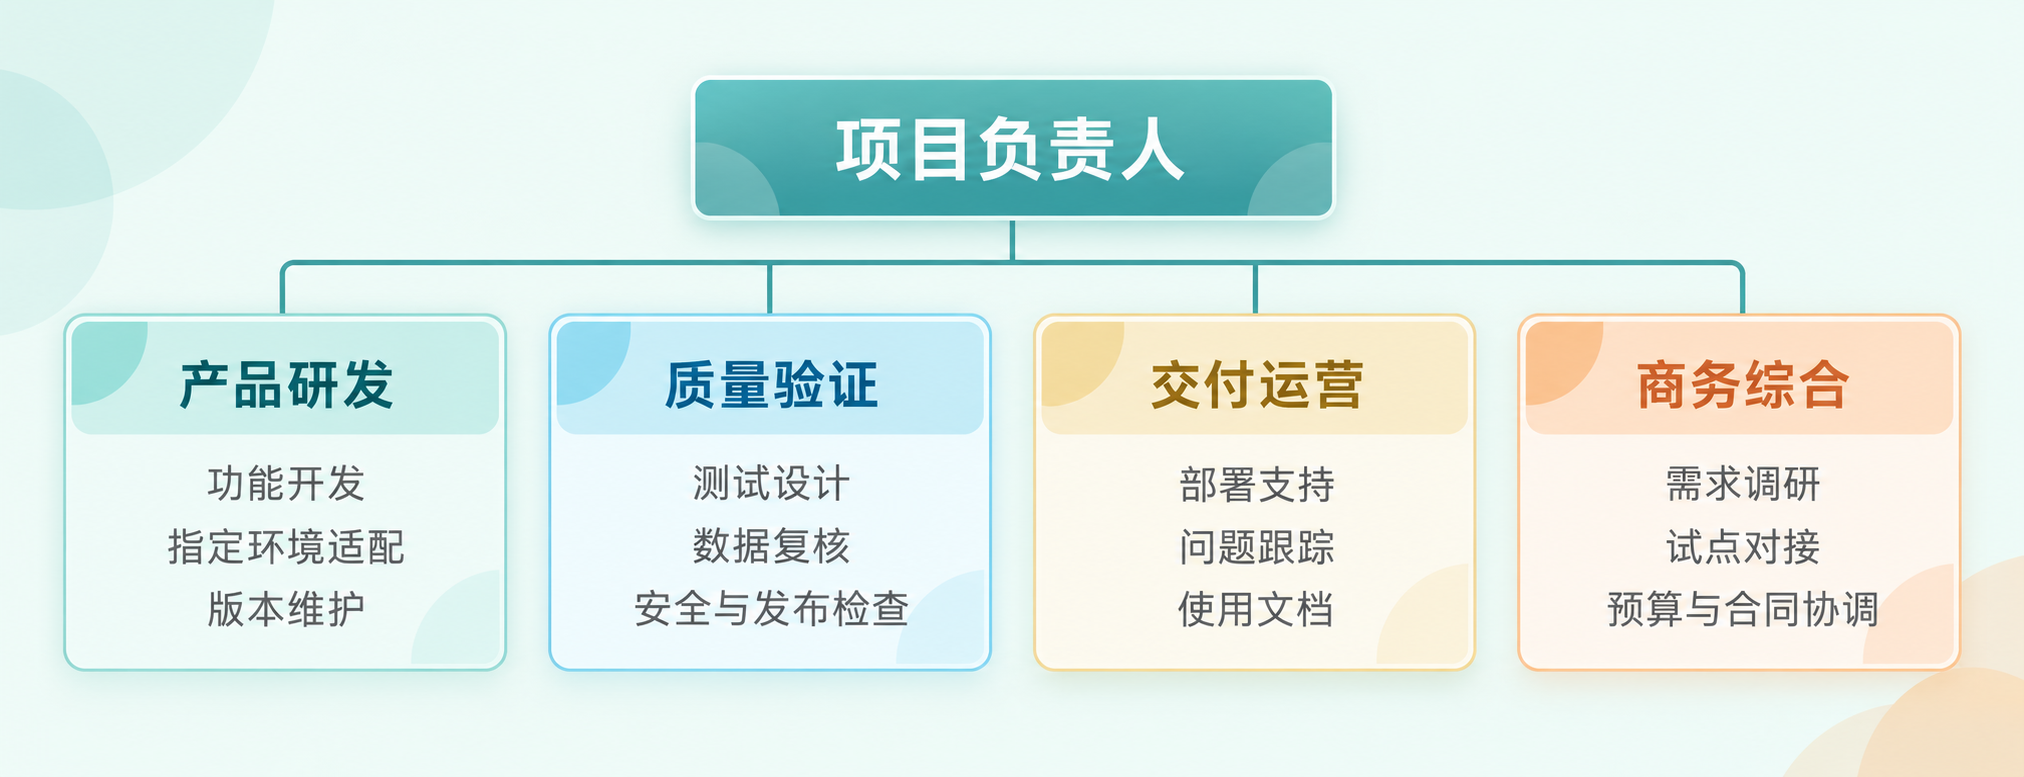
\includegraphics[width=\linewidth,height=.50\textheight,keepaspectratio]{figures/updated-5-3.png}
\caption{创业初期拟定管理架构}\label{fig:5-3}
\end{figure}
\NumberedPara{1}{\textbf{以实际任务配置职责}}
岗位安排依据成员能够独立完成的工作确定。研发职责对应代码与维护记录，质量职责对应测试与复核记录，商务职责对应需求访谈及客户沟通材料。

团队不以职位名称替代实际能力，也不将材料整理工作直接等同于底层技术研发贡献。

\newpage
\NumberedPara{2}{\textbf{建立关键岗位备份}}
关键模块拟同时指定主要负责人和备份人员，定期整理部署方法、常见问题和未完成事项，降低课程安排、毕业或成员流动对项目的影响。

客户环境访问权限、账号及项目资料统一登记；职责变化时同步办理资料和权限交接。

\NumberedPara{3}{\textbf{将培养与交付结合}}
新成员通过环境搭建、测试复现、文档完善和小范围问题修复逐步参与项目。关键修改经评审后合入，避免在缺乏指导和验证的情况下直接影响客户使用。

个人贡献由任务成果、复核质量及协作记录共同体现，不以代码行数或投入时长作为唯一评价标准。

\subsection{创业发展及成熟期管理架构}\label{sec:5.3.2}
随着客户数量和交付规模增长，拟将初期兼任职责逐步拆分为产品研发、质量安全、交付服务、市场商务和财务综合等职能。组织扩展以真实工作量为前提，必要时引入专业外部服务。

\begin{figure}[H]\centering
\setcounter{figure}{3}
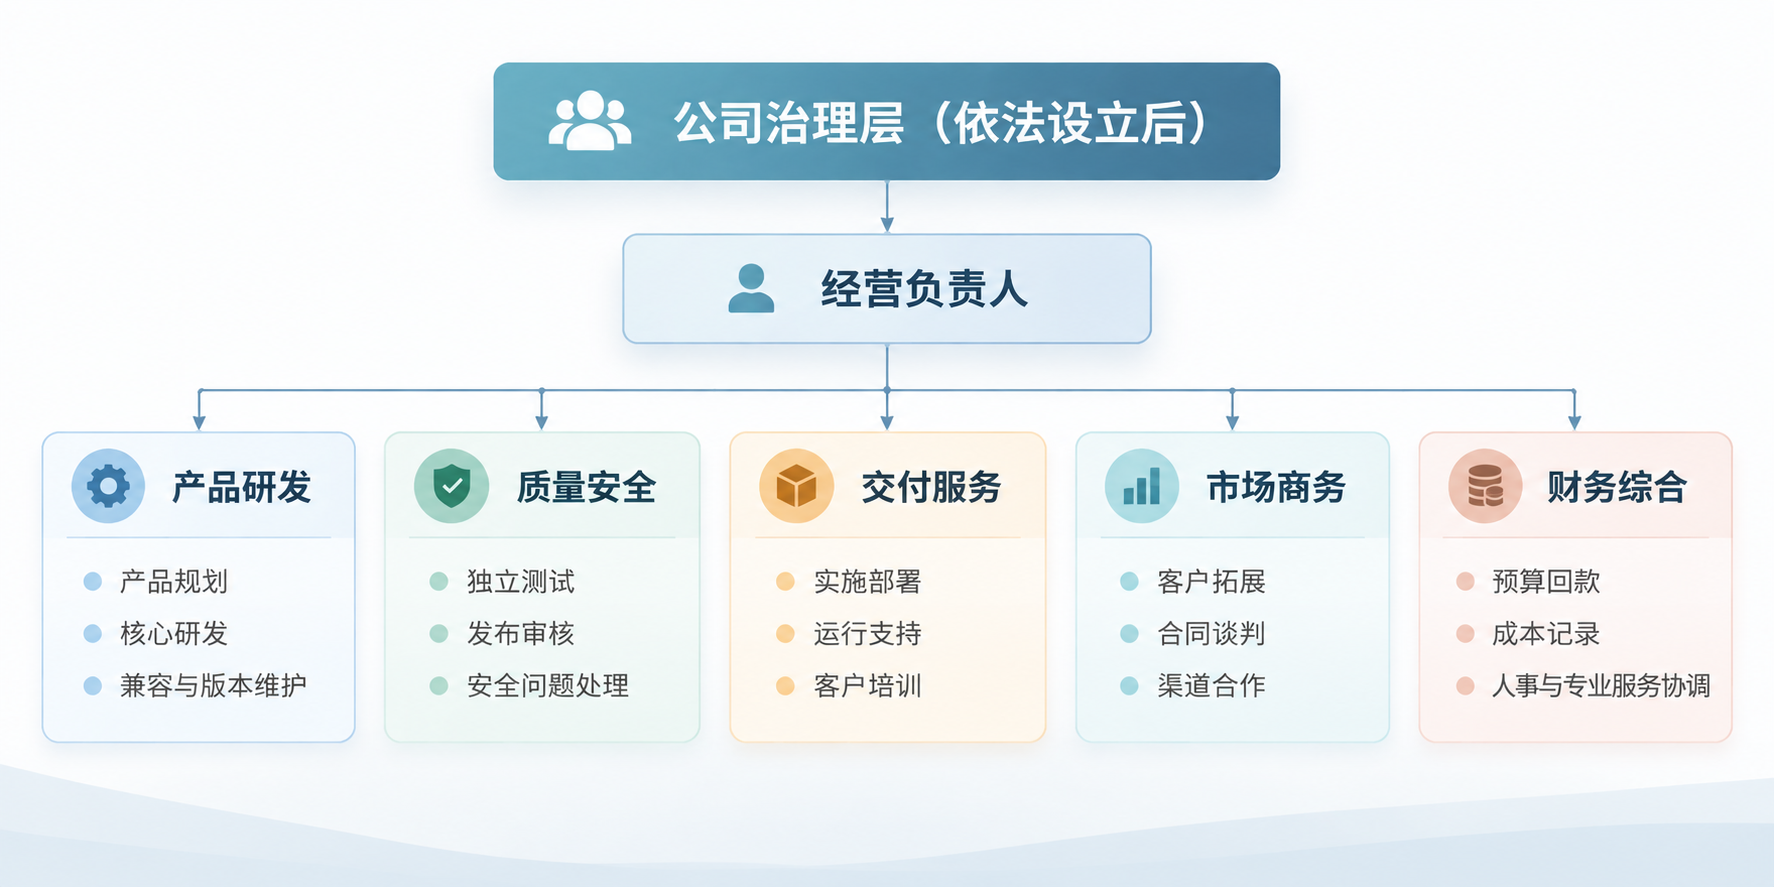
\includegraphics[width=\linewidth,height=.50\textheight,keepaspectratio]{figures/updated-5-4.png}
\caption{创业发展及成熟期拟定管理架构}\label{fig:5-4}
\end{figure}
质量安全职能拟保留重大问题的发布阻断权；销售承诺涉及新增功能、交付期限或服务保障时，由研发和交付共同评估，避免商业承诺超出产品能力。

人员考核围绕部门实际职责展开：研发关注功能质量与维护效率，质量岗位关注问题识别和复核有效性，交付岗位关注验收及问题解决，商务岗位关注有效转化与回款。激励安排综合考虑长期贡献和客户价值，具体薪酬及权益方案在经营主体和资金条件明确后确定。

通过上述安排，PI OS 将逐步形成从需求、研发、测试到交付和服务的责任体系，使技术成果能够稳定转化为客户价值，并为后续创业发展提供组织支撑。

